\chapter{Knowledge Graphs for Cell Communications}
\label{06kg}

\newpage
\section{Introduction}

\begin{figure}
    \centering
    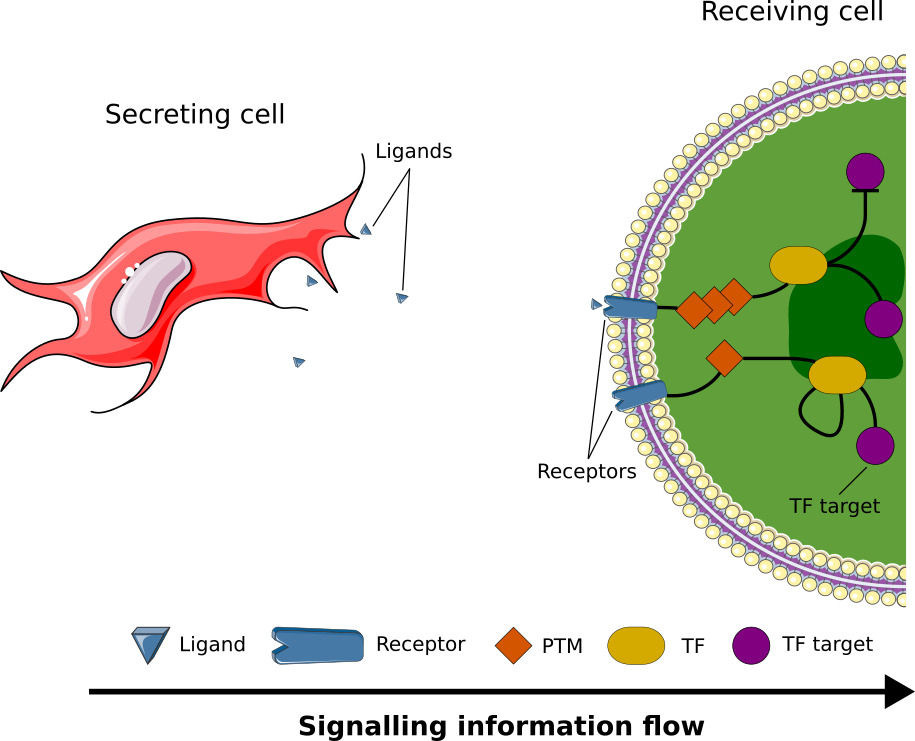
\includegraphics{06kg/figs/6KG_com.png}
    \caption{\textbf{The Directed Nature of Inter- and Intra-Cellular Communications}. Secreting cells interacting with receiving cells via intercellular ligand-receptor interactions, which can then trigger intracellular \acrshort{ptm} cascades and gene-regulatory networks. \acrshort{ptm}, \acrlong{ptm}. \acrshort{tf}, \acrlong{tf}.}
    \label{fig:6intro}
\end{figure}

Cellular signalling involves a complex series of directed and hierarchical~\cite{kumar_3_2003} signal transduction cascades between molecules that dictate a cells response to extrinsic and intrinsic cues. In the context of inter-cellular paracrine communication, a secreting cell produces a series of ligands that are captured by receptors on a receiving cell. The receiving cell then might engage in an intra-cellular signal transduction cascade orchestrated by \acrshort{ptm}s, such as the MAPK cascade~\cite{zhang_mapk_2002}. These cascades regulate gene expression downstream of active transcription factors. With overlapping pathways, feedback loops, and complex settings with multiple cells engaging in symmetrical or non-symmetrical communications, there is nonetheless a directional causality-driven signalling information flow (Figure \ref{fig:6intro}). This directional nature can be measured in terms of graph hierarchy scores, and to aid with that purpose I have developed a python package to compute such scores (Appendix \ref{appendix:pykrack}).

The physical interactions between molecules are often represented as a network of genes, proteins or even \acrshort{ptm}s, described in the manner of a \acrfull{kg}. These network representations have been extensively explored to model both intra- and inter-cellular communications, but to date they are not consistently analysed using methods that leverage the underlying directed and hierarchical nature of signalling processes, often either treating the graph as undirected or analyzing pairwise relationships between feature detection metrics (such as gene expression)~\cite{pratapa_benchmarking_2020, armingol_deciphering_2020}. 
    % Cellular signaling involves overlapping directed \cite{HANCOCK200364} and hierarchical signal transduction cascades between molecules to coordinate targeted behavior \cite{zhang_mapk_2002}.
    % %The physical interactions of molecules are often represented as a network.
    % The resulting network of molecular interactions determines a cell's response under different conditions, drawing interest towards unifying and characterizing varying sources of molecule signaling from distinct scientific experiments. However, methods to represent biological networks and infer gene-gene relationships rarely take into the account the \textit{directionality} and \textit{hierarchical structure} of these gene graphs.

The field of directed cellular interaction databases already presents with some established curated resources like OmniPath~\cite{turei_integrated_2021}, with a growing number of methods attempting to model communication in a directed manner~\cite{lefebvre_large-scale_2021}, describing cell-cell interactions~\cite{fischer_modeling_2022,yang_sctenifoldxct_2023}, and even data-driven \emph{de novo} generation of signal transduction networks~\cite{hu_cytotalk_2021}.

In this chapter I propose a novel approach for assembling gene-gene graphs that capture cellular communication by leveraging \acrshort{kg} embedding approaches, which would allow for the encoding of the original directed \acrshort{kg} into a simpler non-directed format amenable to downstream analysis and data projection. I aim to project single-cell \emph{omic} profiles into the assembled \acrshort{kg}s, thus treating the cells as signals on a gene graph. The resulting signals can then be considered as another single-cell \emph{omic} view of the cells, and used to generate new embeddings or be compared against their gene expression profiles.

This work was conducted in collaboration with Prof. Smita Krishnaswamy and Aarthi Venkat at Yale University, under the Yale-UCL Exchange Programme (\url{https://www.grad.ucl.ac.uk/yale-ucl/}).

        % Gene embedding methods are growing , so are graph signal processing approaches. 
        % Discuss the embedding methods of these graphs:
        % Complexity in terms of structure, directionality and type of interaction. All of this is very important, unlike in undirected knn grpahs ubiquitous to omic analyses.
        % This means that we need some methods able to compute all of this complex relations in multi relation directed graphs  (MultiDiGraph). methods have been developed, transE \cite{bordes_translating_2013}family, graph convolutional networks, and the stuff from he stanford dawn group on  hyperbolic embeddings  \cite{chami_hyperbolic_2019} and general ML approaches applied to non euclidean spaces.
        % Non-euclidean space like hyperbolic spaces argued to be key because graphs with important hierarchical structure [as is biological signalling] is much better capture in a hyperbole than in a plane \cite{bronstein_geometric_2017,nickel_poincare_2017,chamberlain_neural_2017}.[the first one is general Euclidean =bad, the later ones refer to the cocnept of hierarchical graph better on hyperboles than planes].
        % on the other hand, prelim results in collab porject suggest perhaps not as important for bio KG despite the hierarchical nature of signalling networks.



\section{A Knowledge Graph for Ligands, Receptors and TF Targets}

\begin{figure}
    \centering
    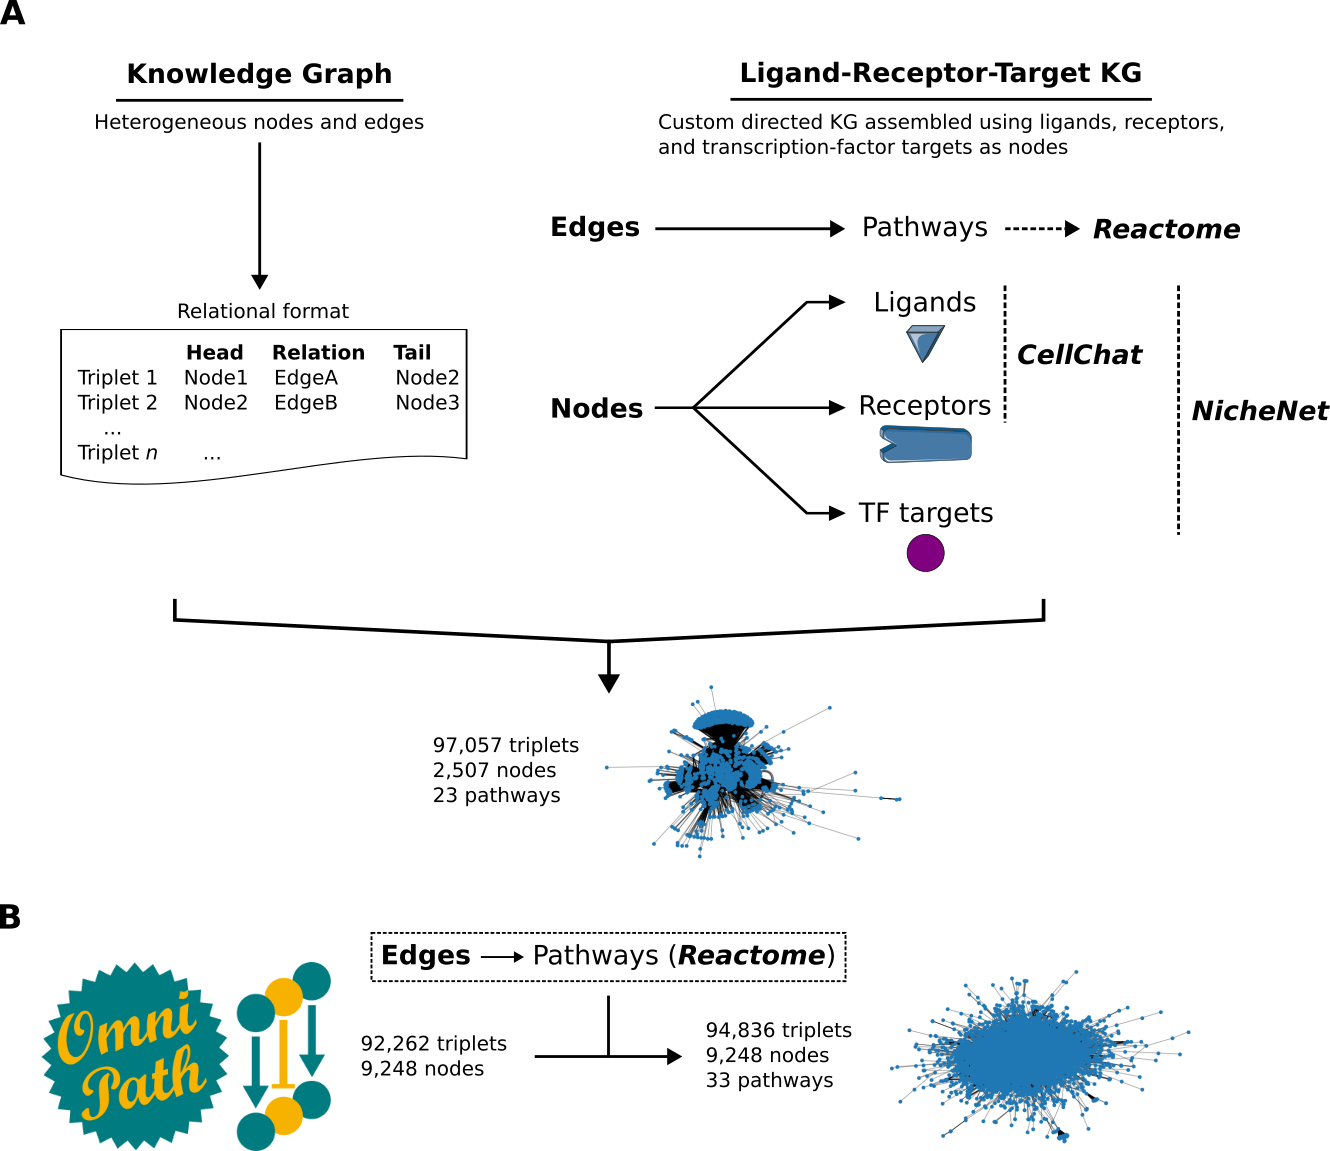
\includegraphics{06kg/figs/6KG_kg.png}
    \caption{\textbf{Assembly of \acrshort{kg}s for Cell Communications.} \textbf{A)} Public databases are used to assemble a custom KG of ligands, receptors and \acrshort{tf} targets. \textbf{B)} Tabular OmniPath~\cite{turei_integrated_2021} repository can also be assembled as a comparable \acrshort{kg}. \acrshort{kg}, \acrlong{kg}. \acrshort{lrtkg}, \acrlong{lrtkg}.}
    \label{fig:6kg}
\end{figure}

Literature information on cell communication interactions is commonly found in the form of databases used for cell-cell communication analyses, and not in a directed graph format. Therefore I assembled a custom \emph{kg} from public databases and compared it with OmniPath~\cite{turei_integrated_2021}, an existing curated repository of directed inter- and intra- cellular signalling interactions. More details on this process can be found in Chapter \ref{02methods}.

I gathered information from the CellChat~\cite{jin_inference_2021} and NicheNet~\cite{browaeys_nichenet_2020} databases to assemble a directed \acrshort{kg} wherein nodes are genes for ligands, receptors or \acrfull{tf} targets (Figure \ref{fig:6kg}). This \acrshort{kg} aims to capture inter- and intra-cellular communication; with ligand and receptor nodes describing the relationship between interacting cells, and the \acrshort{tf} targets capturing cellular states and response to stimuli.

Following the ubiquitous triplet format, I thus encoded the graph as a relational database where pathways from Reactome~\cite{gillespie_reactome_2022} were used to annotate and relate the different gene nodes (Figure \ref{fig:6kg}).

The resulting ligand-receptor-target \acrshort{kg} (\acrshort{lrtkg}) has over 2,500 nodes linked by interactions belonging to 23 distinct pathways. To validate broad-scale graph characteristics this custom graph was compared against the OmniPath resource.
The OmniPath database has multiple layers of relational information between genes (and other molecules such as \acrshort{ptm}s), including directionality, supporting evidence, and functional information on the nature of the interaction (i.e. activation or inhibition of receiving interaction member)~\cite{turei_integrated_2021}. Assembled in the same manner as the LRT-KG object, the OmniPath graph presented with a higher number of gene nodes and pathways but comparatively less interactions  and a lower hierarchy score than the LRT-KG (Figure \ref{fig:6kg}B and Table \ref{tab:2kg}).


\section{KG Embeddings Preserve Graph and Biological Information}

\begin{figure}[H]
    \centering
    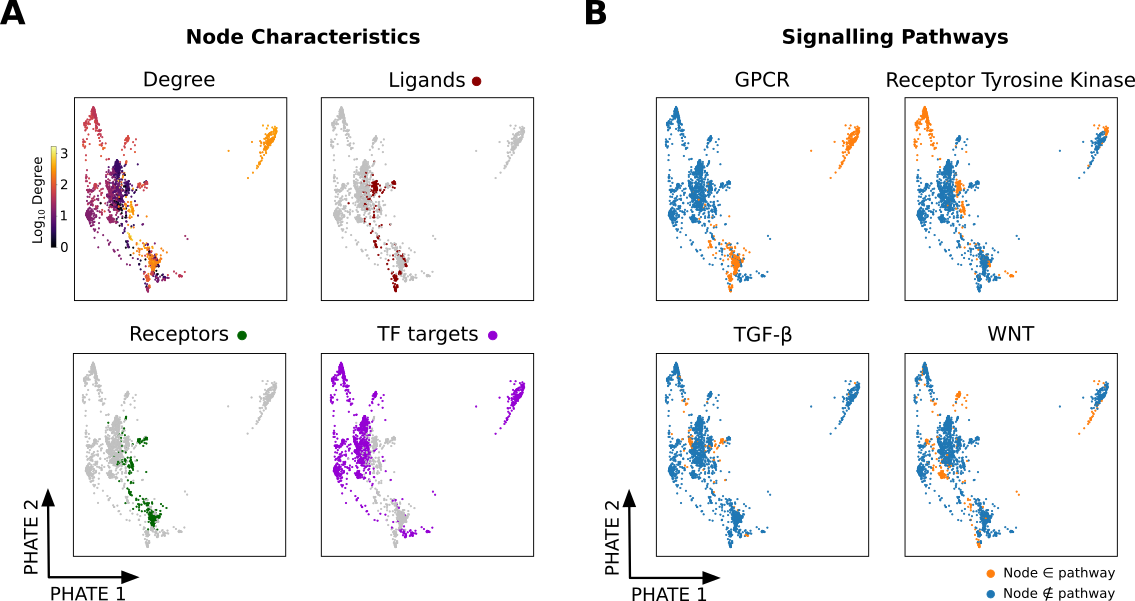
\includegraphics{06kg/figs/6KG_embed.png}
    \caption{\textbf{Information Preservation in Low-Dimensional \acrshort{kg} Embeddings.} \textbf{A)} PHATE of embedded \acrshort{kg} nodes coloured by node-intrinsic properties. \textbf{B)} PHATE of embedded \acrshort{kg} nodes coloured by relational signalling annotations. GPCR, G protein-coupled receptors.}
    \label{fig:6embed}
\end{figure}

To capture the complex relational information in a simpler format amenable to downstream analyses, directed heterogeneous knowledge graphs can be embedded into low dimensional tabular representations. Methods like the classical TransE~\cite{bordes_translating_2013} and its derivatives, graph convolutional networks, and hyperbolic embeddings~\cite{chami_hyperbolic_2019}, represent some of different approaches to learn the structure of \acrshort{kg}s.

I used the TransR method~\cite{zhang_transr_2021} to embed the LRT-KG into a 50-dimensional space (Chapter \ref{02methods}), whose PHATE representation suggests that the embedding method captures topological differences between the distinct node types in the graph (Figure \ref{fig:6embed}A). Node degree also seems to drive some of the topology in the PHATE representation of the embedding, and it would appear that TF targets are the most promiscuous nodes with higher degrees, followed by receptor nodes and finally ligands (Figure \ref{fig:6embed}A). However, care must be taken when making these comparisons for three node classes are imbalanced.

Functional biological information encoded by the edges seems to also be captured in the embedded graph. Signalling pathways belonging to the Signal Transduction category in Reactome, which should cover all three types of node in the LRT-KG, were mapped to gene node embedding. The resulting distribution of pathways, occupying discrete and specific regions of PHATE representation (Figure \ref{fig:6embed}, appears to suggest that relational information from the \acrshort{kg} is also conserved in the 50-dimensional embedding.

% Finally, embedding representation of relations (edges) can be generated, which should capture relations between pathways. Recover high level groupins of pathways with similar biological function, due to their shared nodes on KG.
%     WE can also check out the different pathawys they belong to and see if there is come kind of biologically driver distribution here re pathways. Edges can also be embedded and hopefully lowere level pthawys belonging to a shared bigger levl pathways might lie in closer together? Also deppening on the ratio of shared interactions members between disticnt pathways. 

\section{Projecting Cells as Signals on the KG}

\begin{figure}
    \centering
    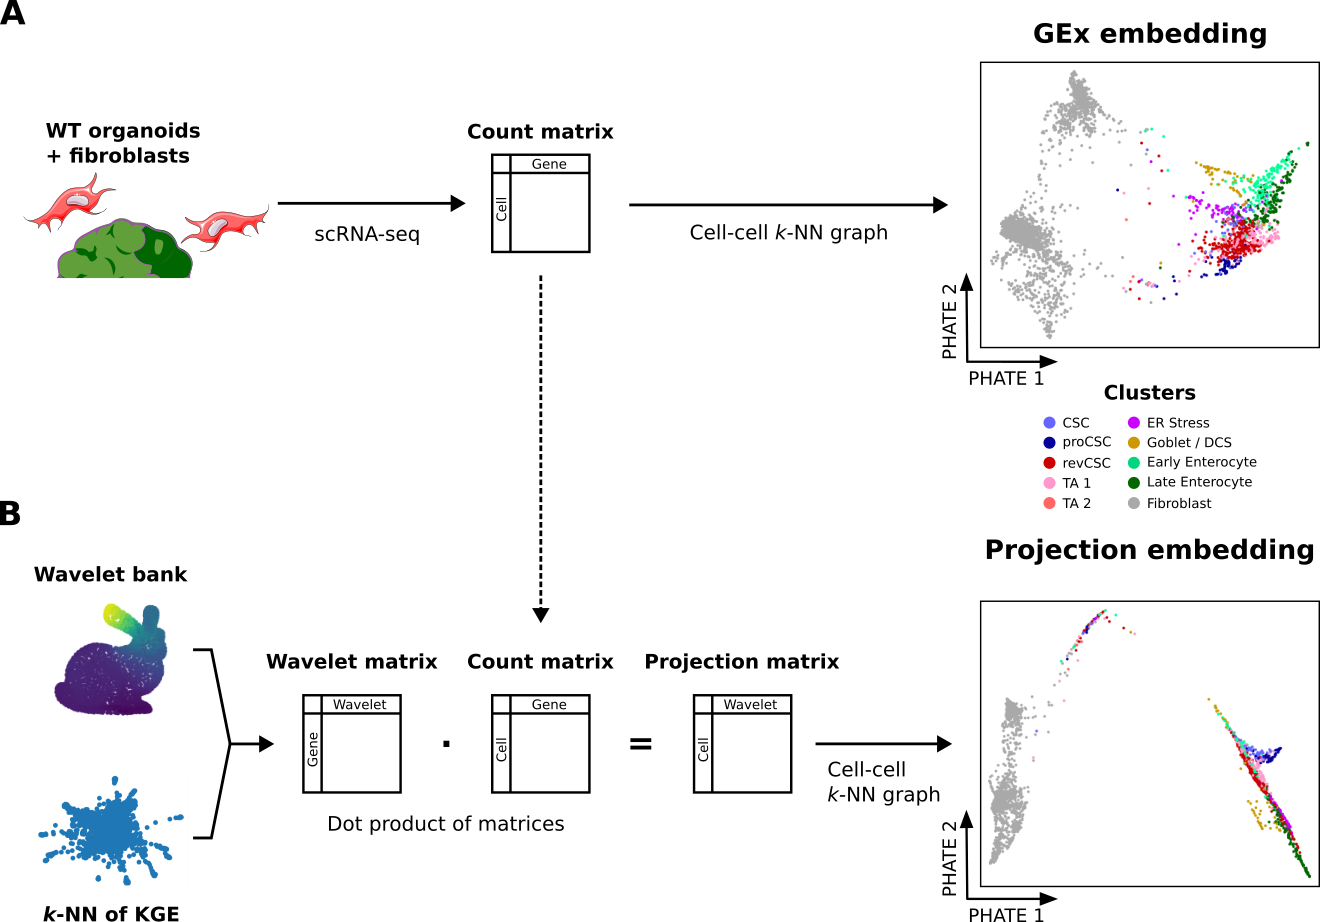
\includegraphics{06kg/figs/6KG_projection.png}
    \caption{\textbf{Projection of \acrshort{gex} Profiles on the \acrshort{lrtkg}.} \textbf{A)} \acrshort{scrnaseq} datasets of \acrshort{wt} organoid and fibroblast co-cultures are used for the projection. \textbf{B)} Wavelet diffusion is applied to the \acrshort{lrtkg} to generate a \(node X wavelets\) matrix onto which the sequencing data is projected. Colours on PHATE plots represent cell clusters.}
    \label{fig:6project}
\end{figure}

Using a WT organoid and fibroblast co-culture scRNA-seq dataset from Chapter \ref{04seq} (Figure \ref{fig:6project}A) I could explore the usefulness of the LRT-KG embedding to describe a cell's \acrfull{gex} profile as projected on a cell communication graph. 

That particular dataset was employed because I had previously established, using cell-cell communication analysis tools and subsequent \acrshort{mc} validation by Dr. Xiao Qin~\cite{cardoso_rodriguez_single-cell_2023} (see Chapter \ref{04seq} for Figure \ref{fig:4cc}A), that the fibroblast cells engage in active communication with the organoid cells, in particular toward the \acrshort{revcsc} state and adjacent areas of the colonic stem compartment. 

When the transcriptomic data is used to generate a PHATE embedding the two distinct cell types are easily resolved, and so are the heterogeneous cell states within the colonic organoid epithelia (Figure \ref{fig:6project}A).

To project these cellular \acrshort{gex} profiles on the LRT-KG I first applied a diffusion wavelet transform to a \emph{k}-NN representation of the LRT-KG embedding, thus generating a \(node X wavelets\) matrix where the first axis corresponds to the gene nodes of the LRT-KG (Figure \ref{fig:6project}B). 

Leveraging the shared feature axis between the \(node X wavelets\) and scRNA-seq \(cell X gene\), I used the dot product (\(\cdot\)) operation to project the transcriptomic data as a \(cell X wavelets\) matrix representation (Figure \ref{fig:6project}B). The projected data can be treated as the scRNA-seq count matrix from above to compute cell-cell \emph{k}-NN graphs and two-dimensional embeddings.

The resulting projection seems to non-quantitatively resemble the \acrshort{gex} profile on a PHATE space, wherein cell type is easily resolved. There appears however that there is some signal loss during the projection process, for epithelial heterogeneity is reduced (Figure \ref{fig:6project}B). 

To quantitatively asses the projection results I not only compared it with the \acrshort{gex} data but also with the interaction strength predictions between cluster pairs in the data (see Chapter \ref{02methods} for more details). 

Average distances between cluster pairs in the LRT-KG projected space and the \acrshort{gex} space were computed based on their \emph{k}-NN representations (Figure \ref{fig:6bench}A) and found to be highly correlated (Figure \ref{fig:6bench}B). A weak positive correlation (\emph{R} = 0.42) between interacting cluster pairs and their distances was observed both in the \acrshort{gex} and highly similar projected spaces (Figure \ref{fig:6bench}C).

Finally, the inter-cluster distance matrices (Sup. Tables \ref{tab:kgdistge} and \ref{tab:kgdistlrt}) were scaled and subtracted to compare the differences between the \acrshort{gex} and projected profiles. Results revealed no distance shortening after projection between the highly interacting fibroblast and \acrshort{revcsc} or \acrshort{ta} clusters. Instead, projection lowered relative distances around the secretory cells and magnifying distances between the \acrshort{ta} and ER stress states (Figure \ref{fig:6bench}D).

In summary these results suggest an insufficient diffusion step prior to data projection, as shown by the similarities between the \acrshort{gex} and projected spaces, and a small degree of signal loss, eroding some the transcriptomic signal unique to secretory cells.

\begin{figure}
    \centering
    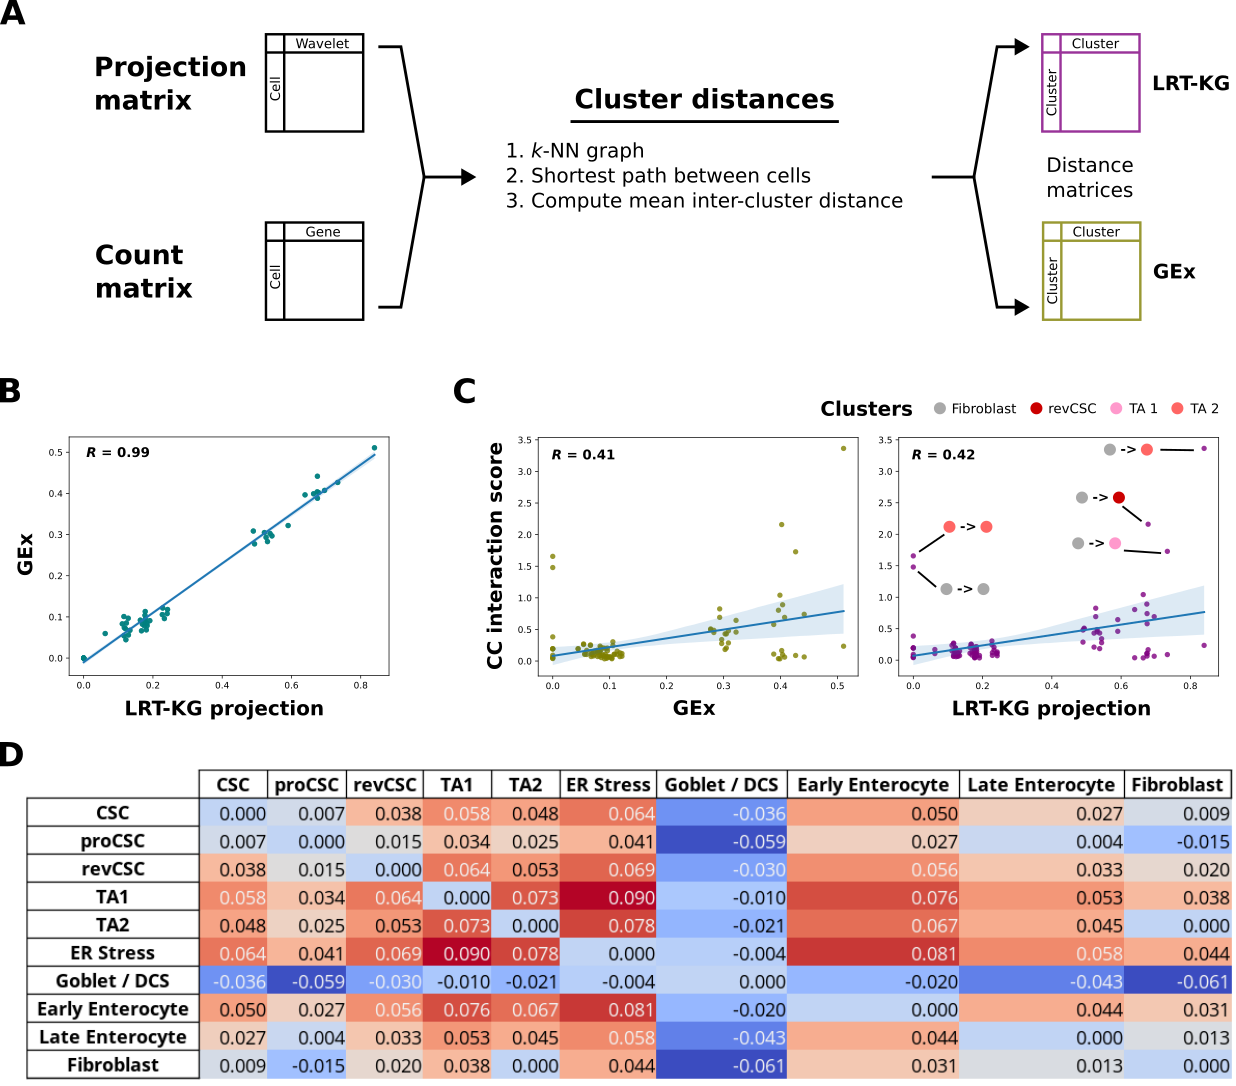
\includegraphics{06kg/figs/6KG_bench.png}
    \caption{\textbf{Comparison of \acrshort{gex} and \acrshort{lrtkg} Projected Profiles.} \textbf{A)} Inter-cluster distances are computed on \acrshort{gex} and projected spaces. \textbf{B)} Correlation between the two distance spaces. \textbf{C)} Correlation between cell-cell communication interaction scores and the distance spaces. Colour annotations reflect highly interacting cluster pairs. \textbf{D)} Scaled differences between the two cluster spaces. Cells are coloured according to the distance difference between a pair of cluster. R, Pearson correlation score.}
    \label{fig:6bench}
\end{figure}

\newpage
\section{Conclusions}

% * Built LRT KG that is comparable to other directed graphs in literature.
%     * IF omnpath capture ground bio truth, cell commns are indeed mostly hierarhcical. WE have a simplified hyper hierarhcical version.
% * KG embedding methods seem to conserve biological properties associted with nodes.
% * Wavelets used to difusse signal on graph so that single-cell \emph{omic} data can be projected on it.
% * Results match/conserve broader GEx information, but information gain is limited regarding cell communications.
% * Need to improve signal difussion step. Alternative gene embedding step can also be explored (GSP paper), so can the benchmarking be improved.


In this chapter I have assembled a \acrlong{kg} for cell communication that captures relational information between ligands, receptors and downstream targets of transcriptional factors. The assembled LRT-KG is comparable in size and graph characteristics to the curated OmniPath database, albeit with a lower number of nodes but enhanced hierarchical structure due to the reductionist approach of limiting signalling flow into a single direction from secreting to receiving cells and the latter's intra-cellular responses. 

From this complex heterogeneous directed LRT-KG, methods like TransR can learn a lower-dimensional embedding that captures the original node characteristics of the graph and even biological information in the form of signalling pathways encoded in the relations between nodes. 
The resulting LRT-KG embedding is a relatively simple tabular representation of the cellular communications LRT-KG onto which we can project the transcriptomic profile of cells via wavelet diffusion.

Projection results revealed similar PHATE embeddings and high inter-cluster distance correlation between the gene expression and projection spaces, suggesting that the diffusion process within the graph is not of a sufficient degree and remains too reliant on the graph's nodes rather than on its structure. 
While the similarities with the \acrshort{gex} profile do validate the projection approach, and some degree of correlation between both spaces was expected, the lacking diffusion step results in the projected space being unable to differentially capture inter-cellular communications between the interacting stromal and epithelial cells of WT organoid and fibroblast co-cultures.


% Given what we know on fibs interacting with revCSC and TA 2, I would expectd thos differences to be decreased on projected space, and at a mor macro level one might expect that cluster pairs displaying higher aggregate interaction probabilities (as determined by CellChat) should have present with shorter distances in the projected space when compared to the GEx space.

